\section{Auswertung}
\label{sec:Auswertung}

Alle Unsicherheiten wurden mit der Python Bibliothek Uncertainties berechnet.\cite{uncertainties}
Diese Bibliothek arbeitet auf dem Prinzip der Gauß'schen Fehlerfortpflanzung
\begin{equation}
    \Delta y = \sum_{i=1}^n \left| \frac{\delta f(x_1,...,x_n)}{\delta x_i} \right| \Delta x_i \, .
    \label{eq:fehlerrechnung}
\end{equation}

\subsection{Bestimmung der Magnetfeldstärke}
\label{ssec:Bestimmung der Magnetfeldstärke}

Die auf- und absteigende Messung der Magnetfeldstärke $B$ je nach Stromstärke $I$ ergibt die Werte in \autoref{tab:magnet}.

% mit \tableSI
\begin{table}
    \centering
    \caption{Messergebnisse der Eichung des Elektromagneten}
    \label{tab:magnet}
    \begin{tabular}{S[table-format=1.1] S[table-format=3.0]}
        \toprule
        \tableSI{I}{\ampere} & \tableSI{B}{\milli\tesla} \\
        \midrule
        0.0 & 6 \\
        0.5 & 52 \\
        1.0 & 97 \\
        1.5 & 142 \\
        2.0 & 188 \\
        2.5 & 233 \\
        3.0 & 280 \\
        3.5 & 322 \\
        4.0 & 365 \\
        4.5 & 404 \\
        5.0 & 439 \\
        \bottomrule
    \end{tabular}
    \begin{tabular}{S[table-format=1.1] S[table-format=3.0]}
        \toprule
        \tableSI{I}{\ampere} & \tableSI{B}{\milli\tesla} \\
        \midrule
        5.0 & 439 \\
        4.5 & 409 \\
        4.0 & 372 \\
        3.5 & 331 \\
        3.0 & 287 \\
        2.5 & 240 \\
        2.0 & 195 \\
        1.5 & 149 \\
        1.0 & 102 \\
        0.5 & 54 \\
        0.0 & 7 \\
        \bottomrule
    \end{tabular}
\end{table}

Diese Werte sind in \autoref{fig:plot_magnet} veranschaulicht. 
Ebenfalls wird eine Ausgleichsrechnung mithilfe von
\begin{equation}
    B(I) = a \cdot I^2 + b \cdot I + c
    \label{eq:ausgleich}
\end{equation}
und der Funktion curve\_fit aus der Python Bibliothek SciPy durchgeführt. \cite{scipy}
Dies ergibt die Parameter
\begin{align*}
    a &= \SI{-2.3+-0.4}{\milli\tesla\per\ampere\squared} \\
    b &= \SI{99.6+-2.1}{\milli\tesla\per\ampere} \\
    c &= \SI{3.7+-2.2}{\milli\tesla} \, .
\end{align*}

\begin{figure}
    \centering
    \includegraphics[width=\textwidth]{build/plot_magnet.pdf}
    \caption{Plot der Messwerte und Ausgleichskurve der Magnetfeldmessung}
    \label{fig:plot_magnet}
\end{figure}

\subsection{Berechnung der Dispersionsgebiete}
\label{ssec:Berechnung der Dispersionsgebiete}

Zunächst müssen die Dispersionsgebiete $\Delta\lambda_\text{D}$ über \autoref{eq:dispers} berechnet werden.

Die betrachteten Wellenlängen sind
\begin{align*}
    \lambda_\text{rot} &= \SI{643.8}{\nano\meter} \\
    \lambda_\text{blau} &= \SI{480.0}{\nano\meter}
\end{align*}
und die zugehörigen Brechungsindizes sind
\begin{align*}
    n_\text{rot} &= \num{1.4567} \\
    n_\text{blau} &= \num{1.4635} \, . \text{\cite{V27}}
\end{align*}
Die Abmessungen der verwendeten Lummer-Gehrcke-Platte sind 
\begin{align*}
    d &= \SI{4}{\milli\meter} \\
    L &= \SI{120}{\milli\meter} \, .
\end{align*}

Daraus folgen die Dispersionsgebiete
\begin{align*}
    \Delta\lambda_\text{D,rot} &= \SI{48.913}{\pico\meter} \\
    \Delta\lambda_\text{D,blau} &= \SI{26.952}{\pico\meter} \, .
\end{align*}

\subsection{Bestimmung der Wellenlängenaufspaltung}
\label{ssec:Bestimmung der Wellenlängenaufspaltung}

Aus den aufgenommenen Fotos des Interferenzmusters der Lummer-Gehrcke-Platte wird nun die, durch den Zeeman Effekt verursachte, Wellenlängenaufspaltung bestimmt.
Die Fotos sind in \autoref{fig:rot}, \autoref{fig:blau_pi} und \autoref{fig:blau_sigma} dargestellt.

In den Fotos werden die Abstände $\Delta s$ und $\delta s$ der Linien wie in \autoref{fig:bild} angedeutet in Pixeln gezählt.

Mit diesen Werten kann nun über 
\begin{equation}
    \delta \lambda = \frac{1}{2}\cdot\frac{\delta s}{\Delta s}\cdot\Delta \lambda_\text{D}
    \label{eq:delta_lambda}
\end{equation}
die die Wellenlängenaufspaltung der einzelnen Linien berechnet werden.
Die Dispersionsgebiete $\Delta\lambda_\text{D}$ werden aus \autoref{ssec:Berechnung der Dispersionsgebiete} entnommen.
Aus den einzelnen Wellenlängenaufspaltungen $\delta \lambda$ wird dann der Mittelwert $\overline{\delta\lambda}$ berechnet.

Die gemessenen Pixelabstände und die einzelnen Wellenlängenaufspaltungen sind in \autoref{tab:rot}, \autoref{tab:blau_pi} und \autoref{tab:blau_sigma} aufgelistet.
Hiermit ergeben sich die gemittelten Wellenlängenaufspaltungen zu 
\begin{align*}
    \overline{\delta \lambda}_\text{rot} &= \SI{9.33+-0.13}{\pico\meter} \\
    \overline{\delta \lambda}_{\text{blau,}\pi} &= \SI{2.90+-0.07}{\pico\meter} \\
    \overline{\delta \lambda}_{\text{blau,}\sigma} &= \SI{6.27+-0.08}{\pico\meter} \, .
\end{align*}

\newpage

\begin{figure}[ht]
    \centering
    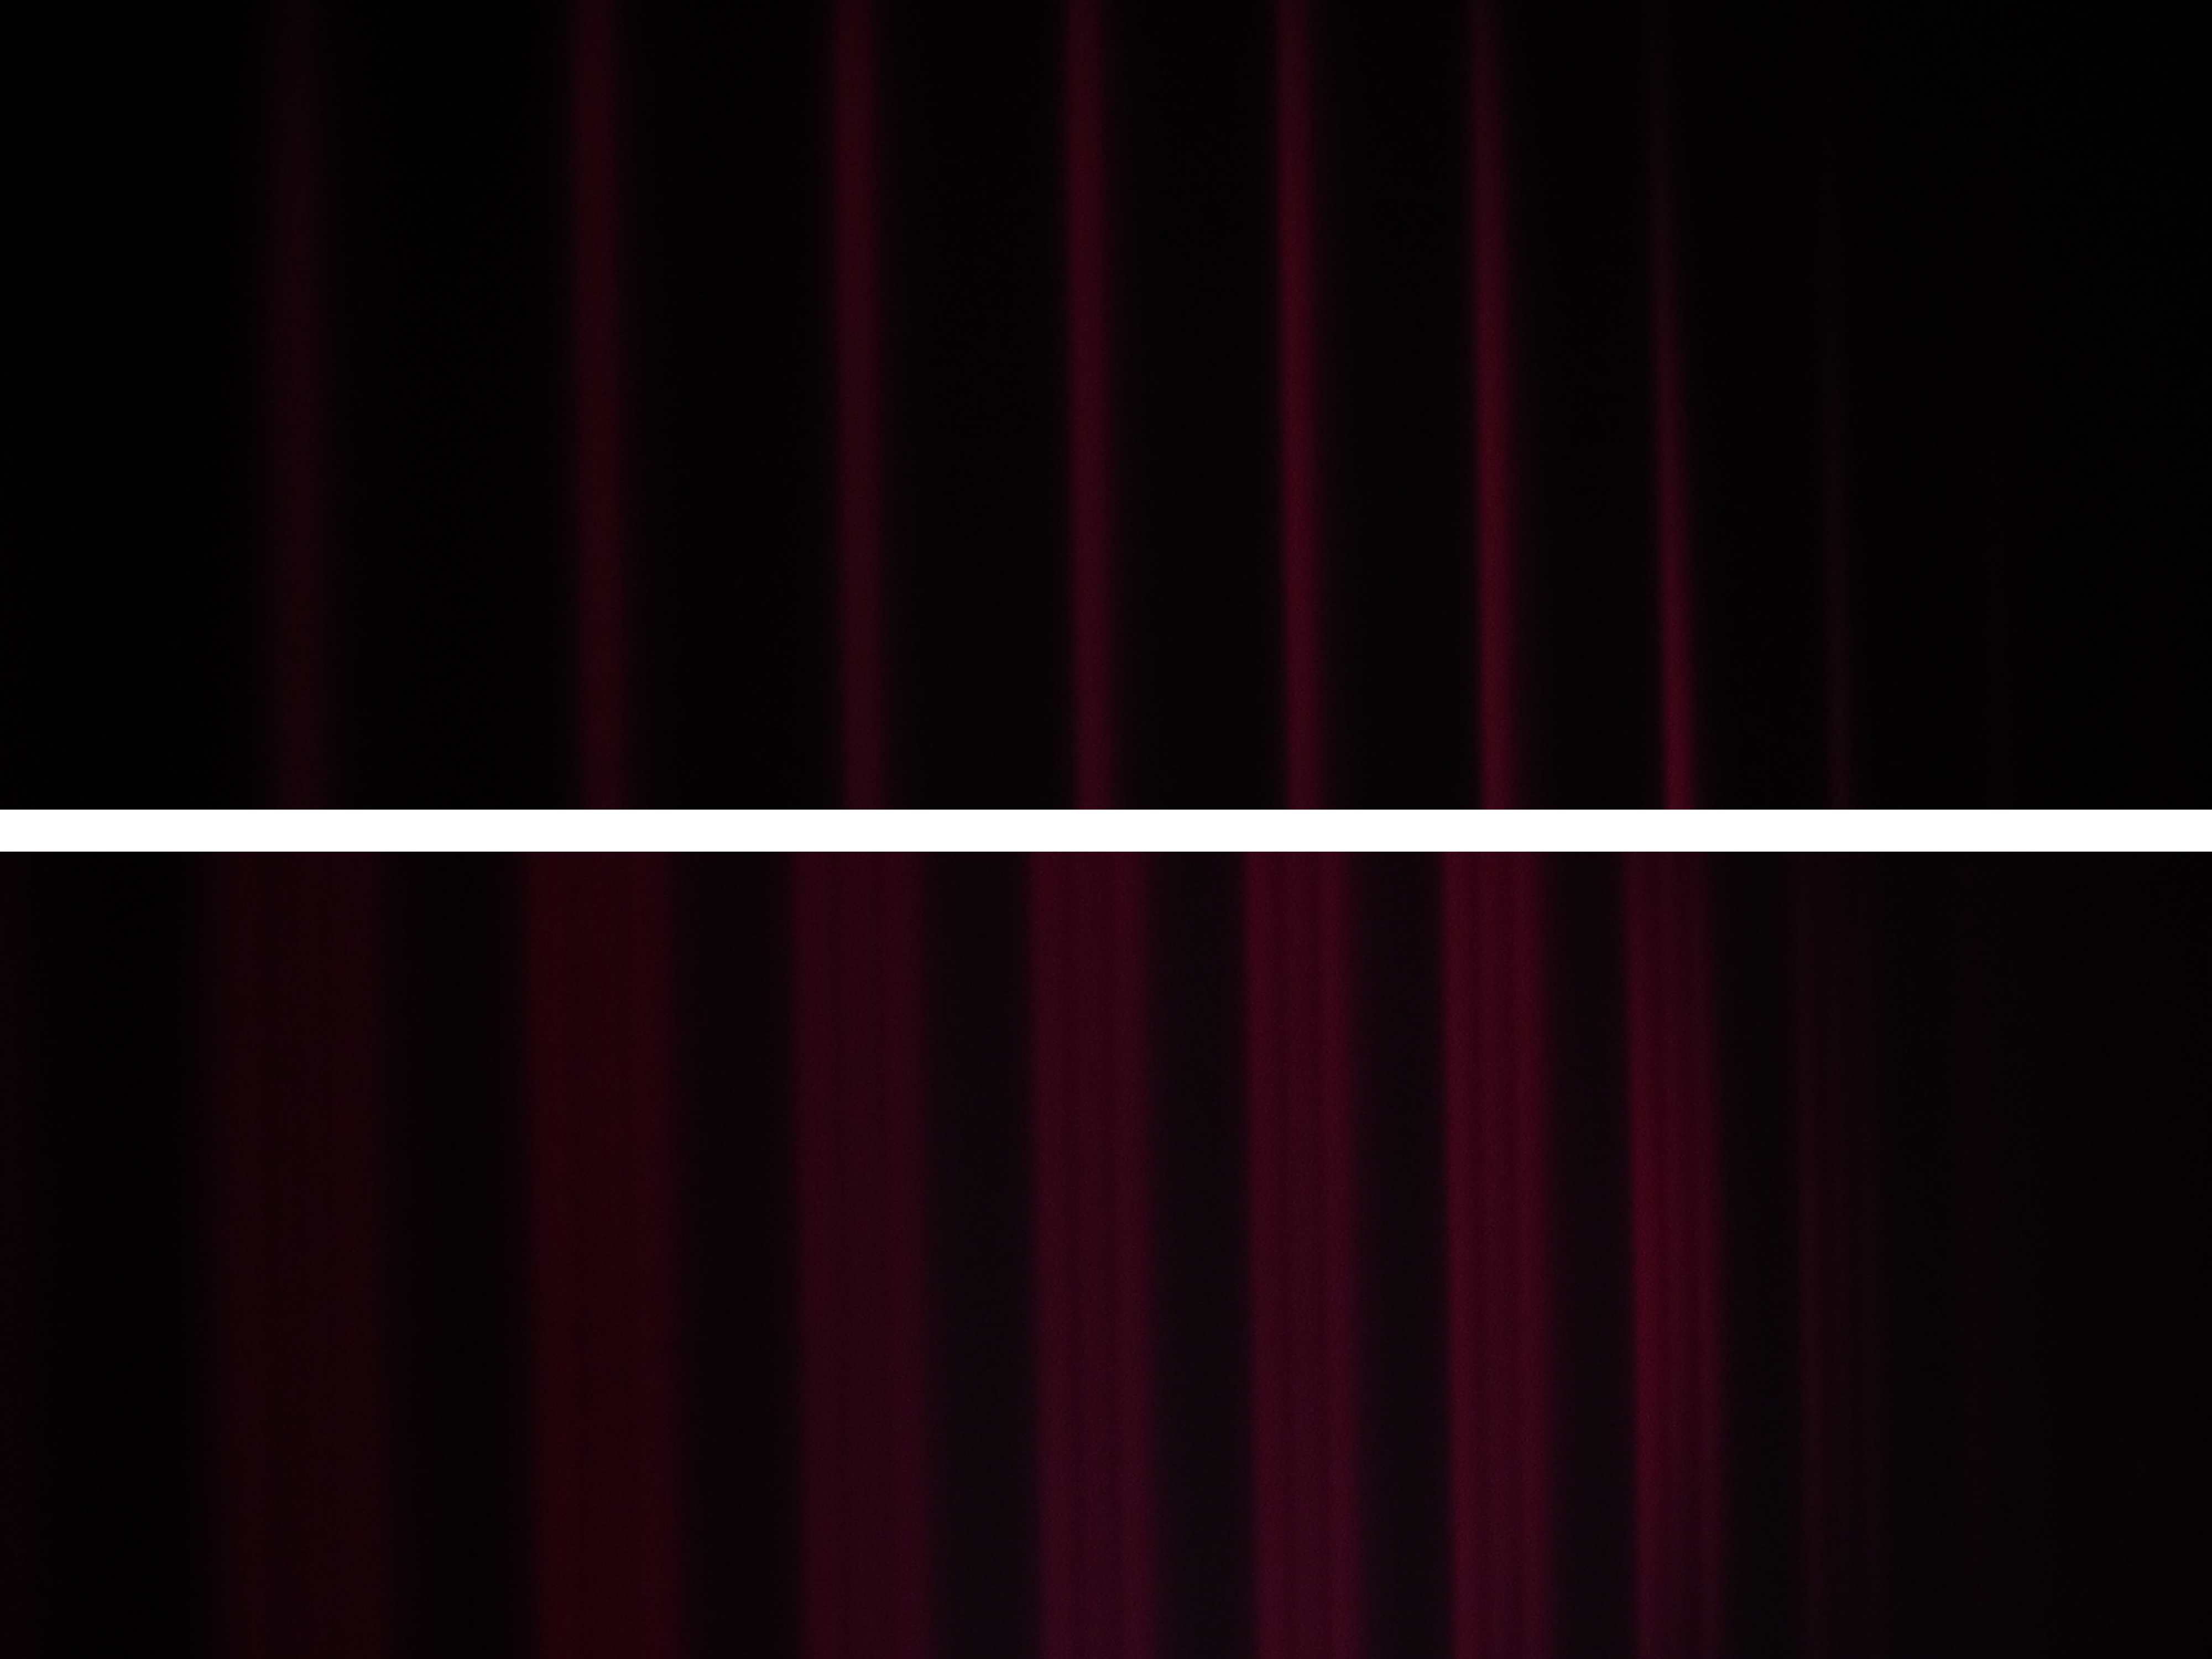
\includegraphics[width=0.8\textwidth]{images/rot.png}
    \caption{Fotos der roten Spektrallinie vor (oben) und nach (unten) der Aufspaltung}
    \label{fig:rot}
\end{figure}

\begin{table}[h]
    \centering
    \caption{Messergebnisse der roten Spektrallinie mit Pixelabständen wie in \autoref{fig:bild} und Wellenlängenaufspaltungen nach \autoref{eq:delta_lambda}}
    \label{tab:rot}
    \begin{tabular}{S[table-format=1.0] S[table-format=3.0(1)] S[table-format=3.0(1)] S[table-format=1.2(3)]}
        \toprule
        \text{Ordnung }n & \tableSI{\Delta s}{Pixel} &\tableSI{\delta s}{Pixel} & \tableSI{\delta \lambda}{\pico\meter}  \\
        \midrule
        1 & 551+-5 & 218+-5 & 9.68+-0.24 \\
        2 & 471+-5 & 178+-5 & 9.24+-0.28 \\
        3 & 416+-5 & 159+-5 & 9.35+-0.31 \\
        4 & 379+-5 & 143+-5 & 9.23+-0.34 \\
        5 & 354+-5 & 134+-5 & 9.26+-0.37 \\
        6 & 333+-5 & 128+-5 & 9.40+-0.39 \\
        7 & 294+-5 & 110+-5 & 9.15+-0.44 \\
        \bottomrule
    \end{tabular}
\end{table}

\begin{figure}[ht]
    \centering
    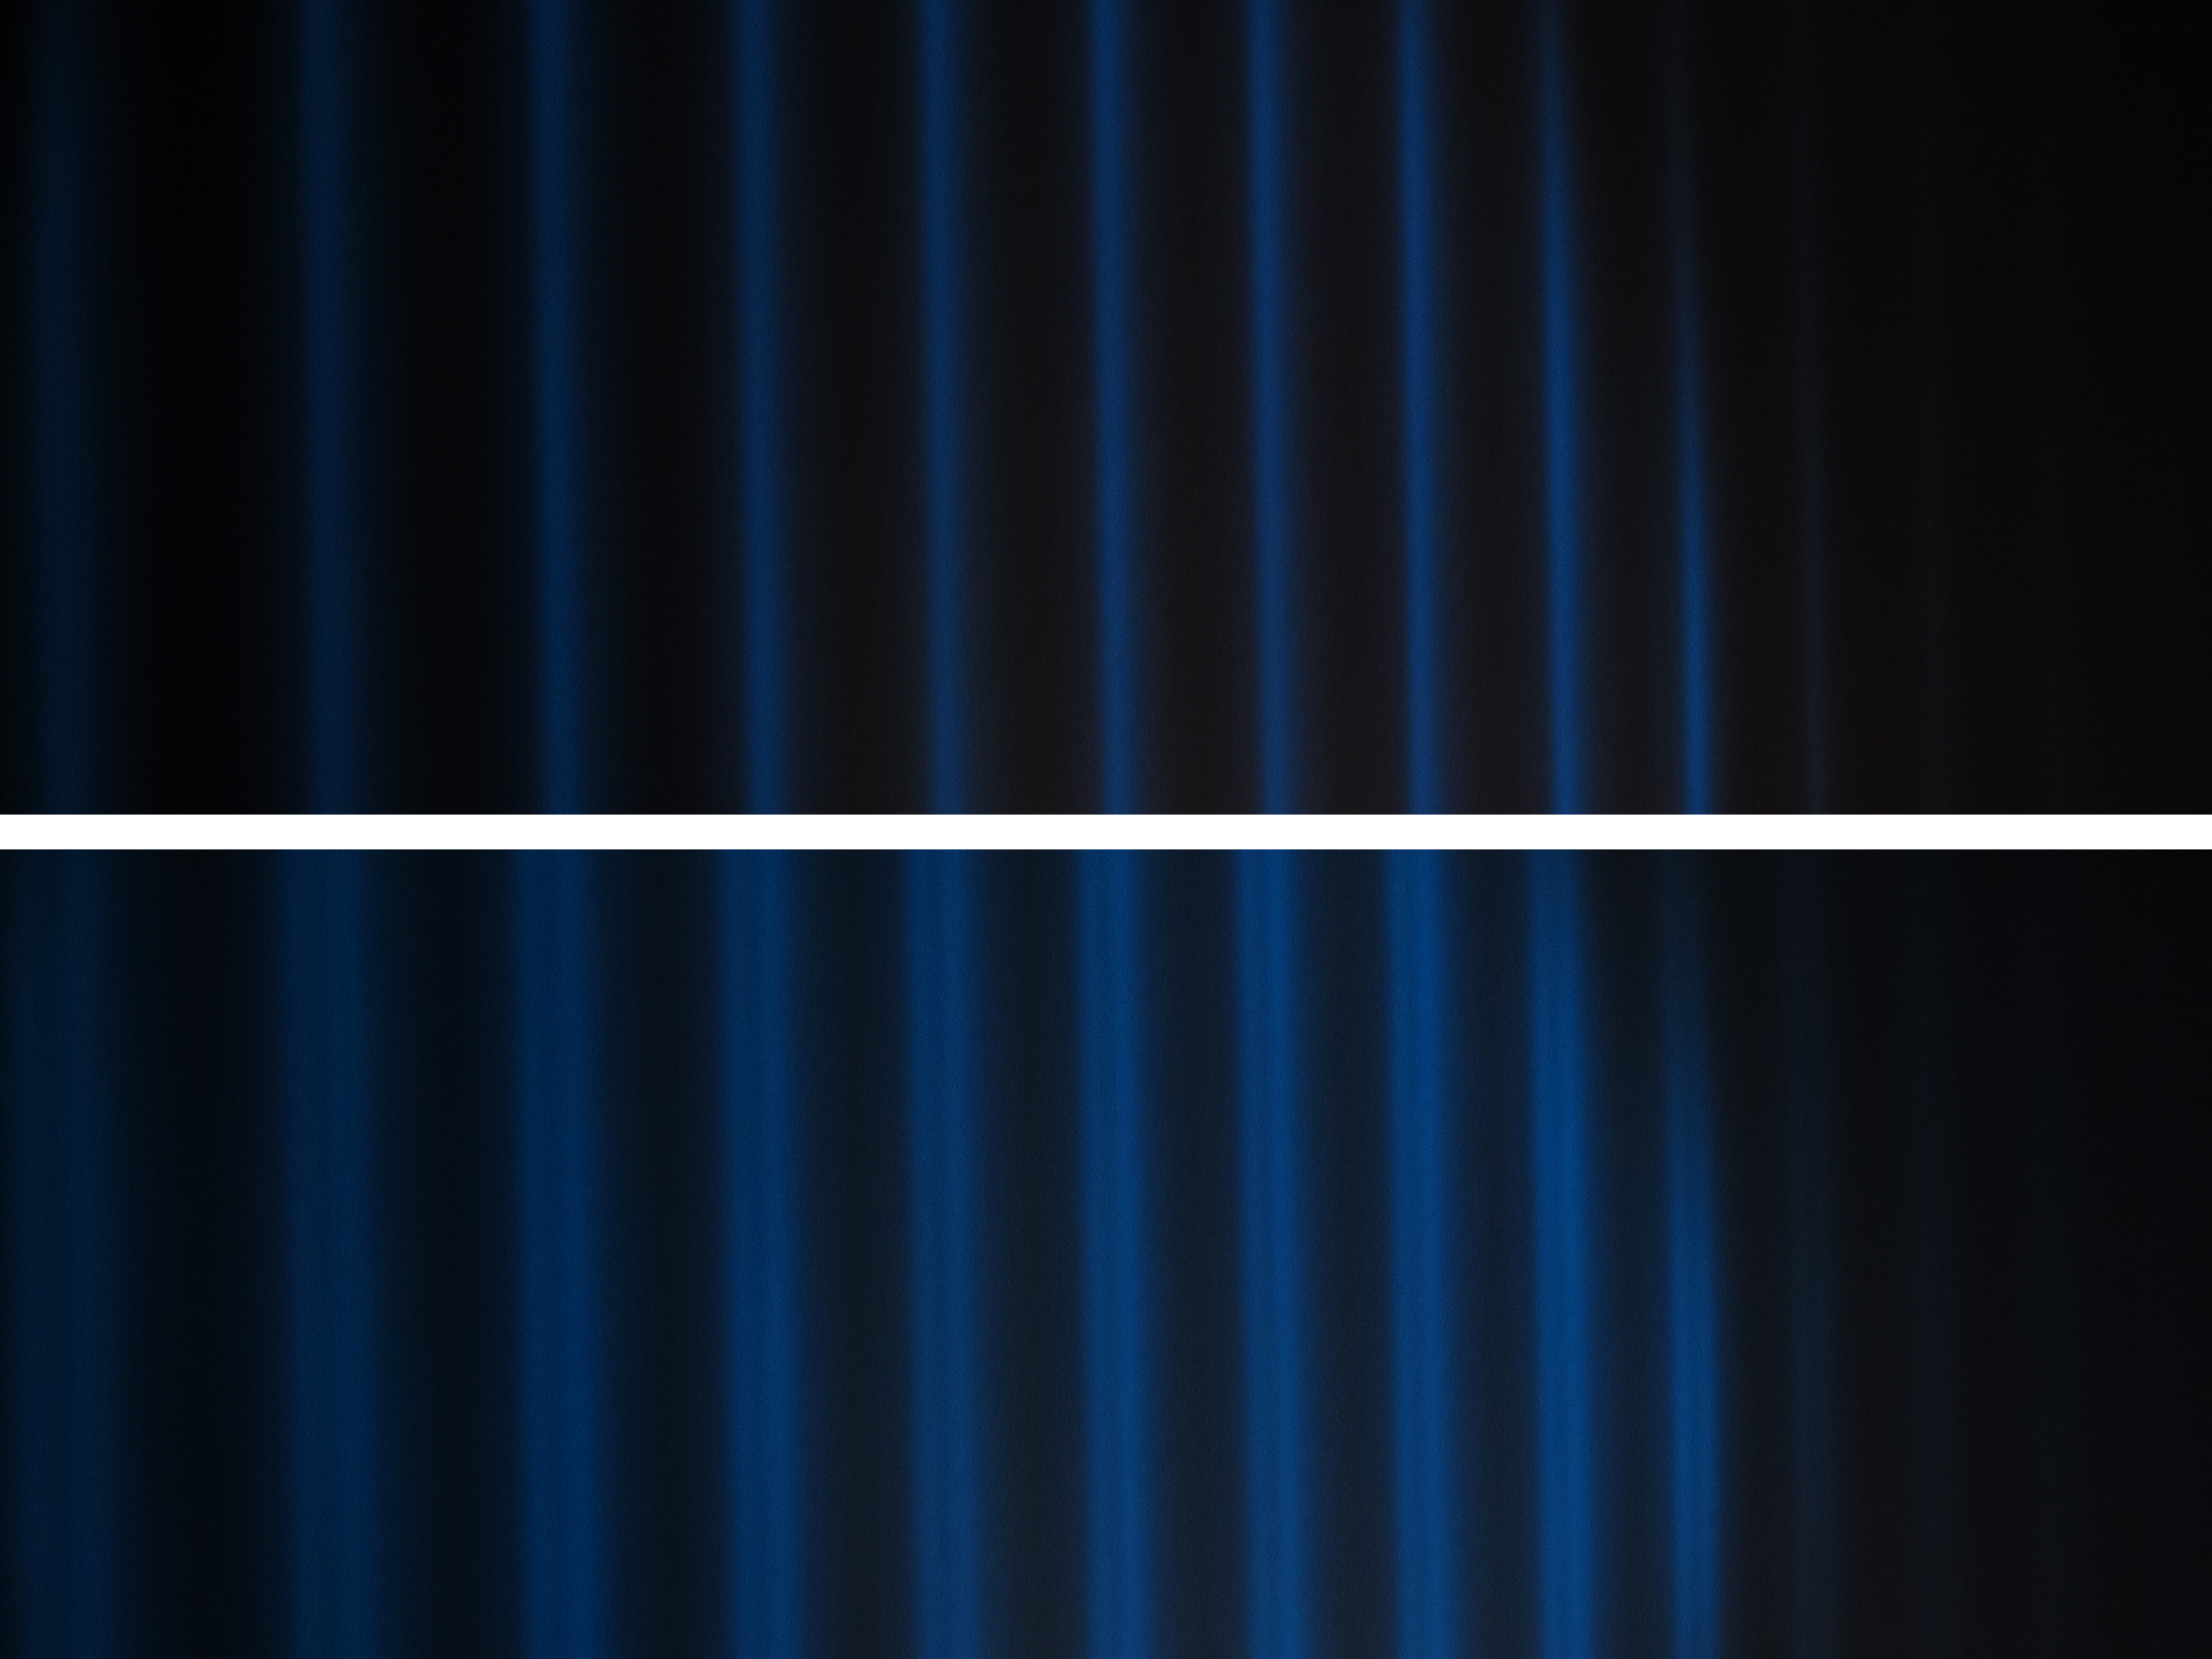
\includegraphics[width=0.8\textwidth]{images/blau_pi.png}
    \caption{Fotos der blauen $\pi$-Spektrallinie vor (oben) und nach (unten) der Aufspaltung}
    \label{fig:blau_pi}
\end{figure}

\begin{table}[ht]
    \centering
    \caption{Messergebnisse der blauen $\pi$-Spektrallinie mit Pixelabständen wie in \autoref{fig:bild} und Wellenlängenaufspaltungen nach \autoref{eq:delta_lambda}}
    \label{tab:blau_pi}
    \begin{tabular}{S[table-format=1.0] S[table-format=3.0(1)] S[table-format=3.0(1)] S[table-format=1.2(3)]}
        \toprule
        \text{Ordnung }n & \tableSI{\Delta s}{Pixel} &\tableSI{\delta s}{Pixel} & \tableSI{\delta \lambda}{\pico\meter}  \\
        \midrule
        1 & 500+-5 & 117+-5 & 3.15+-0.14 \\
        2 & 420+-5 & 84+-5 & 2.70+-0.16 \\
        3 & 370+-5 & 79+-5 & 2.88+-0.19 \\
        4 & 340+-5 & 77+-5 & 3.05+-0.20 \\
        5 & 318+-5 & 68+-5 & 2.88+-0.22 \\
        6 & 291+-5 & 63+-5 & 2.92+-0.24 \\
        7 & 273+-5 & 61+-5 & 3.01+-0.25 \\
        8 & 260+-5 & 56+-5 & 2.90+-0.27 \\
        9 & 244+-5 & 53+-5 & 2.93+-0.28 \\
        10 & 223+-5 & 47+-5 & 2.84+-0.31 \\
        11 & 217+-5 & 42+-5 & 2.61+-0.32 \\
        \bottomrule
    \end{tabular}
\end{table}

\begin{figure}[ht]
    \centering
    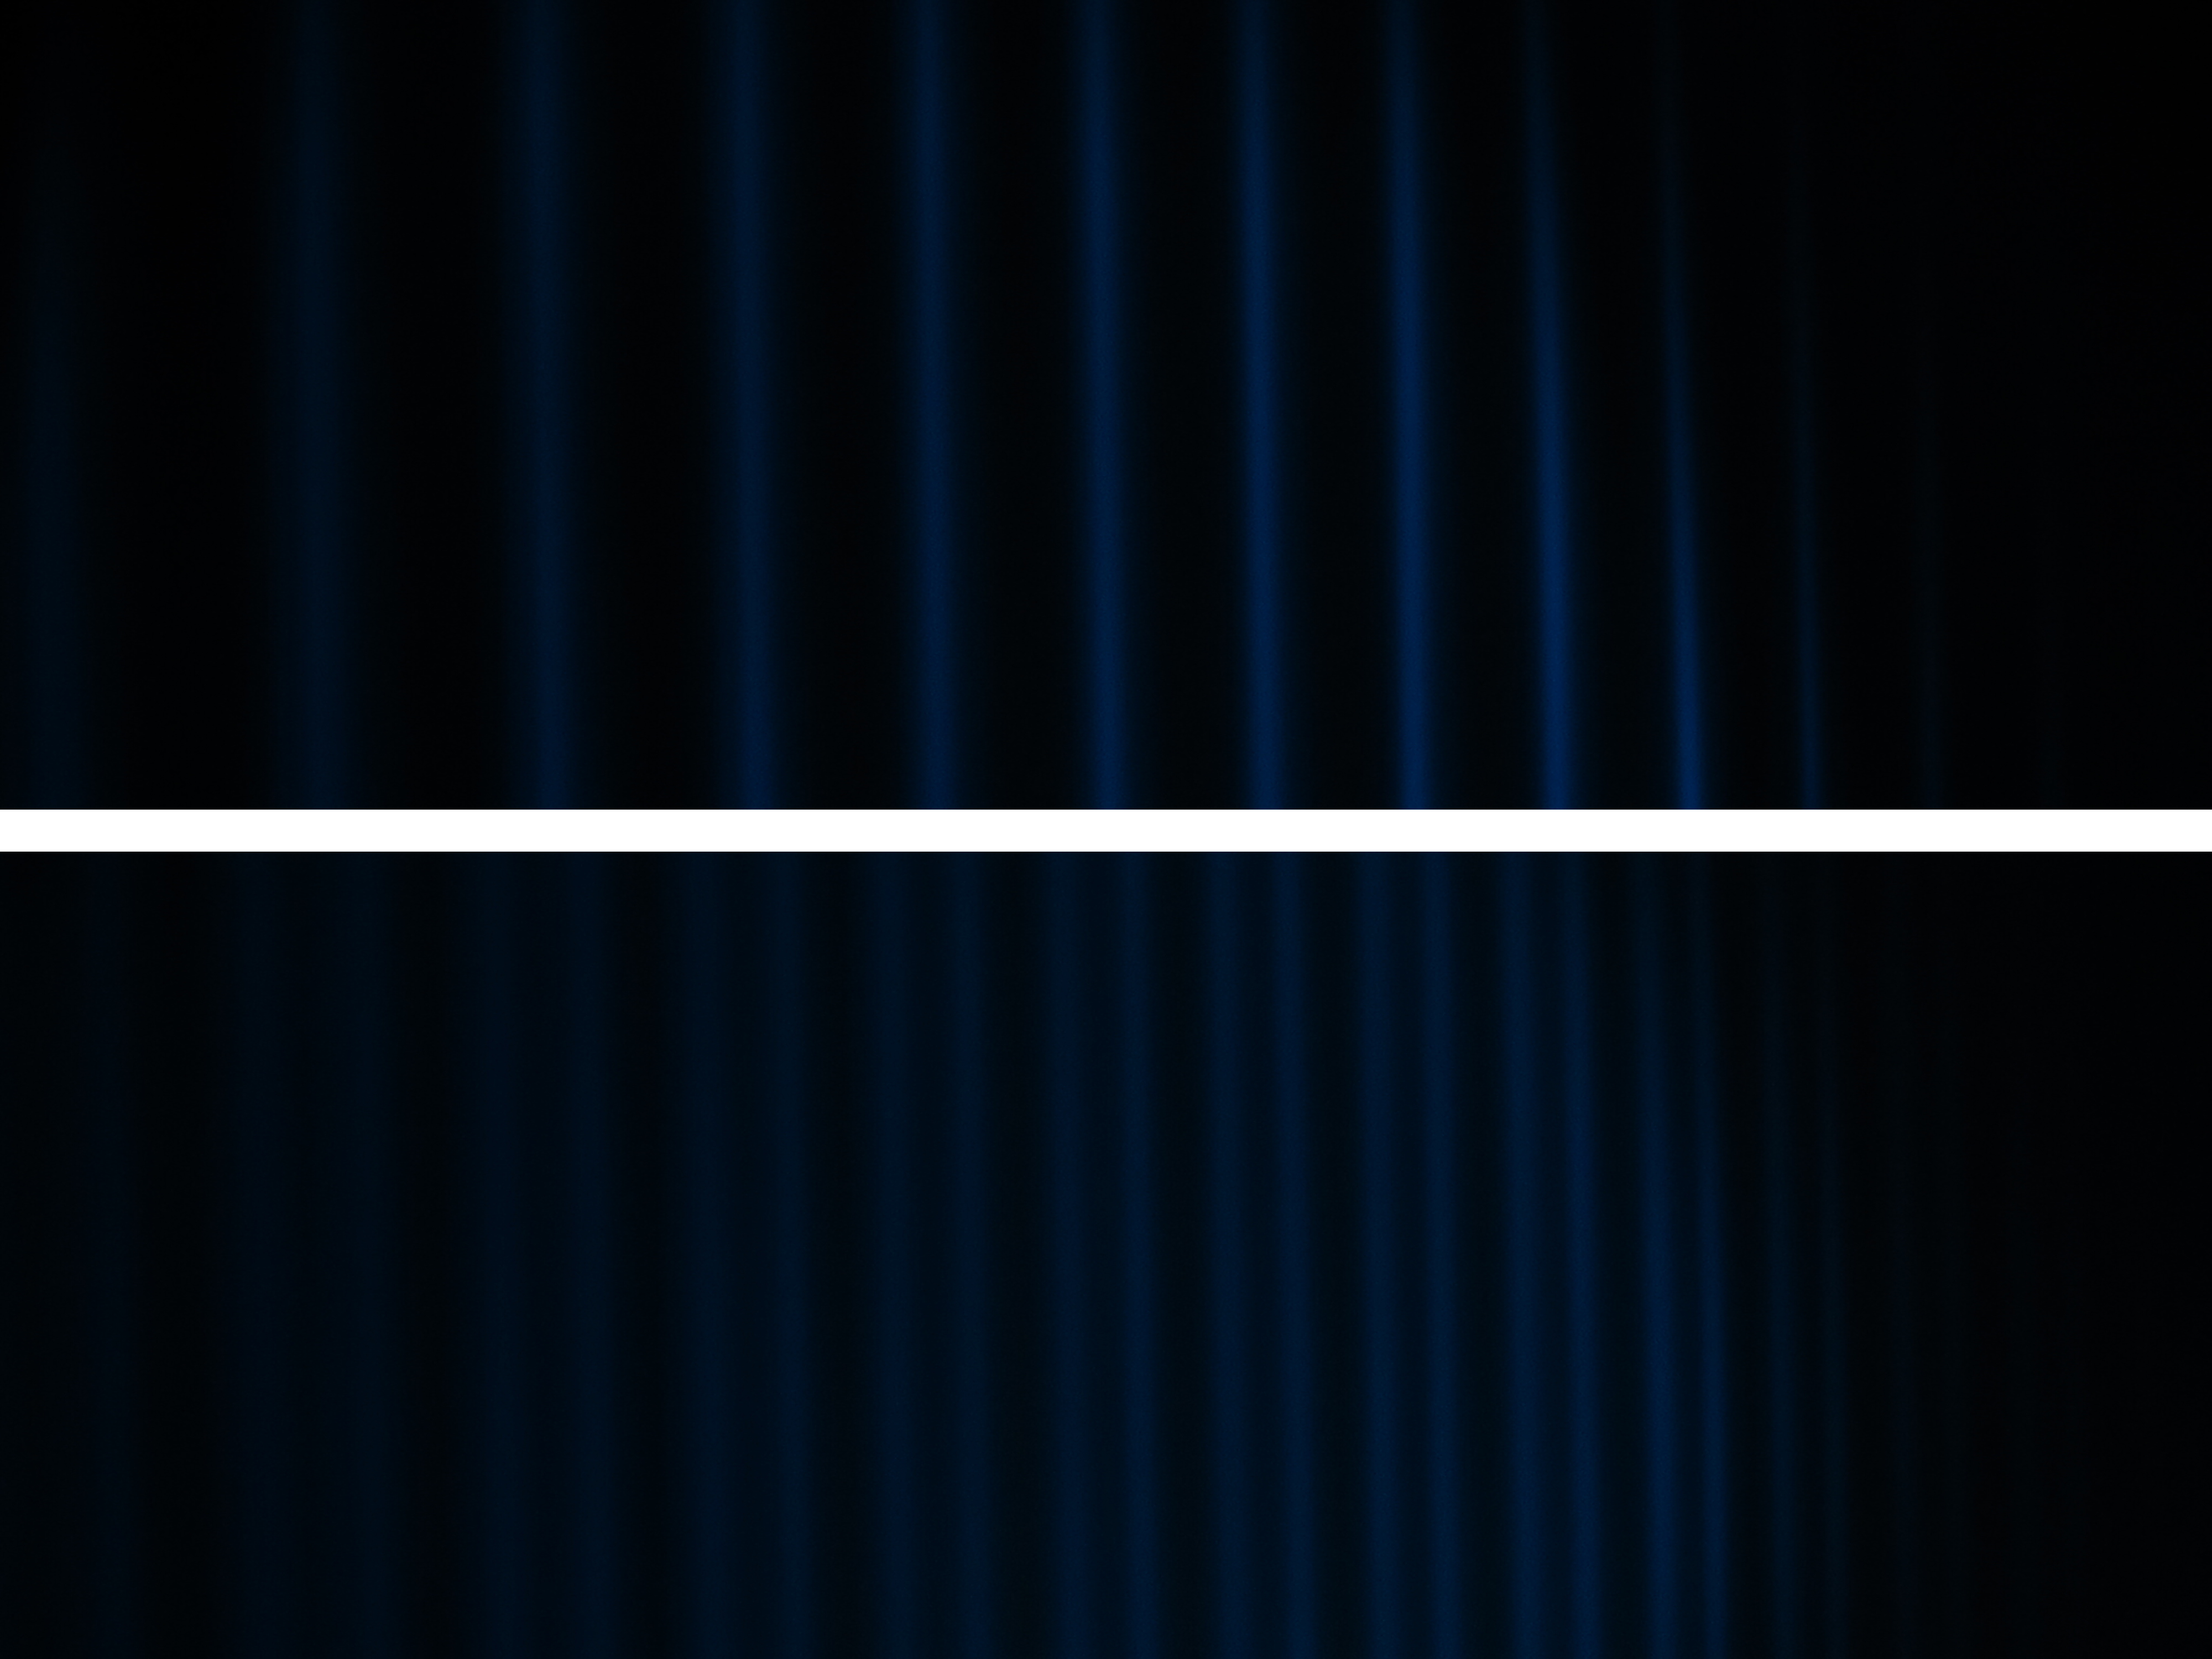
\includegraphics[width=0.8\textwidth]{images/blau_sigma.png}
    \caption{Fotos der blauen $\sigma$-Spektrallinie vor (oben) und nach (unten) der Aufspaltung}
    \label{fig:blau_sigma}
\end{figure}

\begin{table}[ht]
    \centering
    \caption{Messergebnisse der blauen $\sigma$-Spektrallinie mit Pixelabständen wie in \autoref{fig:bild} und Wellenlängenaufspaltungen nach \autoref{eq:delta_lambda}}
    \label{tab:blau_sigma}
    \begin{tabular}{S[table-format=1.0] S[table-format=3.0(1)] S[table-format=3.0(1)] S[table-format=1.2(3)]}
        \toprule
        \text{Ordnung }n & \tableSI{\Delta s}{Pixel} &\tableSI{\delta s}{Pixel} & \tableSI{\delta \lambda}{\pico\meter}  \\
        \midrule
        1 & 506+-5 & 243+-5 & 6.47+-0.15 \\
        2 & 421+-5 & 202+-5 & 6.47+-0.18 \\
        3 & 377+-5 & 179+-5 & 6.40+-0.20 \\
        4 & 330+-5 & 156+-5 & 6.37+-0.23 \\
        5 & 317+-5 & 145+-5 & 6.16+-0.23 \\
        6 & 288+-5 & 129+-5 & 6.04+-0.26 \\
        7 & 271+-5 & 127+-5 & 6.32+-0.27 \\
        8 & 258+-5 & 117+-5 & 6.11+-0.29 \\
        9 & 245+-5 & 114+-5 & 6.27+-0.30 \\
        10 & 225+-5 & 104+-5 & 6.23+-0.33 \\
        11 & 220+-5 & 100+-5 & 6.13+-0.34 \\
        \bottomrule
    \end{tabular}
\end{table}

\subsection{Bestimmung der Landé-Faktoren}
\label{ssec:Bestimmung der Lande-Faktoren}

Die Landé-Faktoren $g_{i,j}$ lassen sich über die umgestellte \autoref{eq:gij} berechnen.
Die Naturkonstanten sind 
\begin{align*}
    h &= \SI{6.626e-34}{\joule\second} \\
    c &= \SI{2.998e8}{\meter\per\second} \\
    \mu_B &= \SI{9.274e-24}{\joule\per\tesla} \, .
\end{align*}

Die Magnetfeldstärken werden über die durchgeführte Ausgleichsrechnung mit \autoref{eq:ausgleich} berechnet.
Die während der Messung verwendeten Stromstärken sind
\begin{align*}
    I_{\text{rot}} &= \SI{5.0}{\ampere} \\
    I_{\text{blau},\pi} &= \SI{5.0}{\ampere} \\
    I_{\text{blau},\sigma} &= \SI{3.24}{\ampere} \, .
\end{align*}
Damit ergeben sich die Magnetfeldstärken 
\begin{align*}
    B_{\text{rot}} &= \SI{443.5}{\milli\tesla} \\
    B_{\text{blau},\pi} &= \SI{443.5}{\milli\tesla} \\
    B_{\text{blau},\sigma} &= \SI{302.1}{\milli\tesla} \, .
\end{align*}
Wobei sich hier die Unsicherheiten zu einer Größe von $10^{-4}\,\si{\milli\tesla}$ ergeben und deswegen nicht weiter beachtet werden.

Nun werden mithilfe der gemittelten Wellenlängenaufspaltungen die Landé-Faktoren zu
\begin{align*}
    g_{i,j,\text{rot}} &= \num{1.086+-0.015} \\
    g_{i,j,\text{blau},\pi} &= \num{0.607+-0.015} \\
    g_{i,j,\text{blau},\sigma} &= \num{1.929+-0.023} \, .
\end{align*}